\section{Bilans opakowań i materiałów pomocniczych}

Kosmetyki rozlewane do butelek wykonanych z materiału bio-PET pochodzącego w 100\% z recyklingu, stworzonego na bazie trzciny cukrowej.

\begin{figure}[h]
	\centering
	\begin{subfigure}[t]{0.45\textwidth}
	\centering
	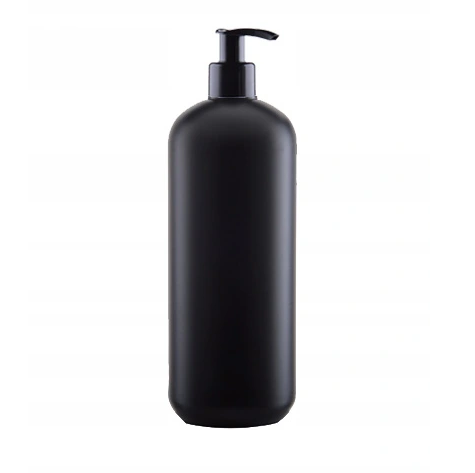
\includegraphics[width=\textwidth]{./sec9/butelka1.png}
		\caption{Dozownik w formie pompki; pojemność: 500\,ml; wymiary 7,4\,cm x 7,4\,cm x 18,6\,cm; waga 35\,g; kolor czarny; ilość w kartonowym opakowaniu zbiorczym 100 sztuk\protect\footnote{\url{https://allegro.pl/oferta/butelka-z-\-dozownikiem-do-zelu-mydla-pompka-500ml-9708856613?bi_s=ads&bi_m=showitem\%3Aactive&bi_c=NjRhY2JkMDYtYzc5MS00MjkxLTlmZDAtM2FhZGI5MzBiMzFjAA&bi_t=ape&referrer=proxy&emission_unit_id=b357113d-ff81-4cbf-93b9-39d19bdc982c}}}
	\end{subfigure}
	\hfill
	\begin{subfigure}[t]{0.45\textwidth}
	\centering
	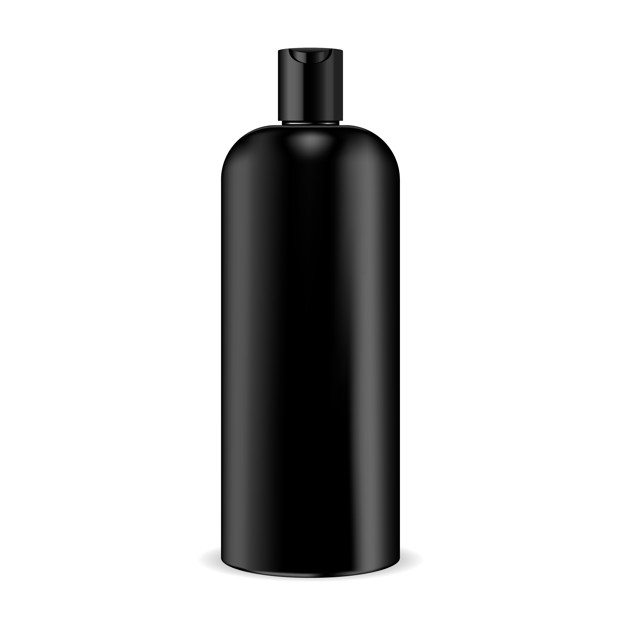
\includegraphics[width=\textwidth]{./sec9/butelka2.jpg}
		\caption{Zamknięcie typu disc cap; pojemność: 300\,ml; wymiary 16,5\,cm x 6,4\,cm x 6,4\,cm; waga 21\,g; kolor czarny; ilość w kartonowym opakowaniu zbiorczym 125 sztuk\protect\footnote{\url{https://www.freepik.com/premium-vector/cosmetic-shampoo-black-bottle-mockup_4188953.html}}}
	\end{subfigure}
	\caption{Butelki na (a) szampony i (b) odżywki}
\end{figure}

\begin{table}[h]
	\centering
	\caption{Etykiety wykonane z papieru metalizowanego. Zapotrzebowanie}
	\begin{tabular}{lllll}
		\hline
		\textbf{Produkt} & \textbf{Produkcja roczna} & \makecell[l]{\textbf{Zapotrzebowanie} \\ \textbf{dzienne}} & \makecell[l]{\textbf{Zapotrzebowanie} \\  \textbf{tygodniowe}} & \makecell[l]{\textbf{Zapotrzebowanie} \\ \textbf{miesięczne}} \\
		\hline\hline
		Odżywka proteinowa & 500 tys. butelek 300ml & \multirow{3}{*}{\makecell[l]{6250 sztuk \\ 50 kartonów butelek}} & \multirow{3}{*}{\makecell[l]{31250 sztuk \\ 250 kartonów butelek}} & \multirow{3}{*}{\makecell[l]{131250 sztuk \\ 1050 kartonów butelek}} \\
		Odżywka emolientowa & 500 tys. butelek 300ml & & & \\
		Odzywka humektantowa & 500 tys. butelek 300ml & & & \\
		\cline{3-5}
		Szampon ziołowy & 660 tys. butelek 500ml & \multirow{2}{*}{\makecell[l]{5500 sztuk\\ 55 kartonów butelek}} & \multirow{2}{*}{\makecell[l]{27500 sztuk \\ 275 kartonów butelek}} & \multirow{2}{*}{\makecell[l]{115500 sztuk \\ 1155 kartonów butelek}} \\
		Szampon peelingujący & 660 tys. butelek 500ml \\
		\hline
	\end{tabular}
\end{table}

